\chapter{Progettazione ed Implementazione su LUNES}

\begin{figure}[H]
    \centering
    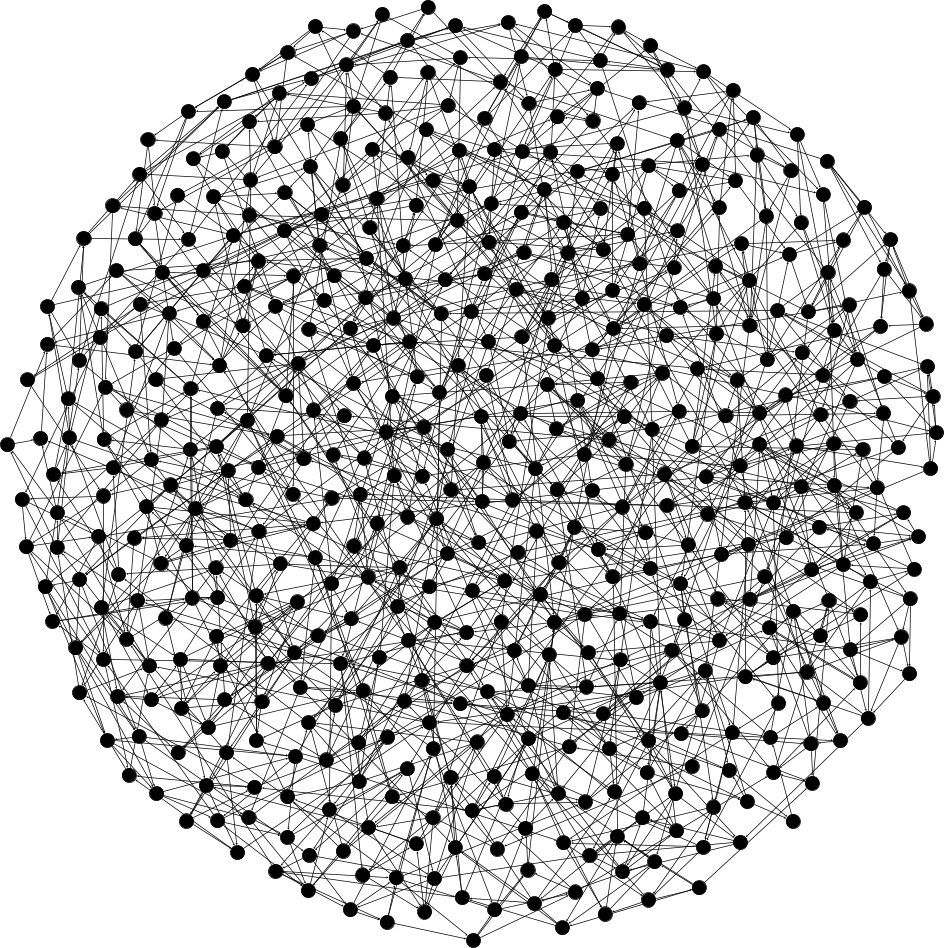
\includegraphics[width=0.6\textwidth]{images/network-500.png}
    \caption{Visualizzazione di una rete di esempio con $500$ nodi e $10000$ vertici generata con \textit{igraph}.}
\end{figure}
\textit{LUNES} permette di costruire una piattaforma ed eventi basata su agenti molto performante, capace di far interagire le varie \textit{Simulated Entities} utilizzando anche il vincolo temporale. Il simulatore, infatti, essendo \textit{time-stepped} permette di utilizzare la componente \textit{tempo} come parte integrante della simulazione. Il tempo all'interno della simulazione non rispecchia quello del mondo reale e permette di valutare dei processi molto lunghi come composti da uno o più \textit{step}. Ad esempio l'operazione di \textit{mining} dei nodi non può essere replicata rispecchiando le tempistiche reali ma conoscendo alcuni parametri è possibile costruirne la funzione di probabilità ed applicarla alla simulazione.\newline
Il simulatore inizialmente si occupa di creare i \textit{peer} ed i collegamenti sulla base di un grafo generato tramite la libreria \href{https://igraph.org/}{\textit{igraph}}. Con la creazione della rete vengono inizializzate anche le strutture dati, usate dai \textit{peer}, per il salvataggio di dati, scambio di informazioni, dati sul proprio stato e della rete. Ogni \textit{Simulated Entity} rappresenta un nodo della rete.\newline
La gestione delle interazioni tra i vari \textit{peer} è gestita come una macchina a stati finita che reagisce ai vari eventi in arrivo dai nodi o prodotti dal nodo stesso. Ogni evento è caratterizzato da una singola azione che il nodo può compiere e quindi questa progettazione modulare risulta essere molto estensibile: per ogni nuova azione aggiuntiva è sufficiente generare la gestione per il singolo evento.\newline
Utilizzando il \textit{Simulation Manager} di \textit{ARTÌS} e \textit{GAIA} non è necessario progettare od implementare i meccanismi di comunicazione e \textit{load balancing} che la progettazione prevede. Una volta creata la rete ed i collegamenti \textit{ARTÌS} è incaricato di consegnare i messaggi (eventi) ai nodi.\newline
\textit{LUNES} fornisce alcune implementazioni dei maggiori algoritmi di \textit{gossip} [\ref{appendix:gossip}] come \textit{broadcast}, \textit{broadcast probabilistico} e \textit{broadcast dipendente dal grado}. Non è presente però l'algoritmo \texttt{Dandelion} utilizzato nella reale implementazione dei client per Bitcoin. Questa mancanza non risulta essere bloccante in quanto è dimostrato\cite{gdalunes} che le implementazioni degli algoritmi di \textit{gossip} messi a disposizione da \textit{LUNES} consentono di raggiungere il $100\%$ di copertura della rete con un ridotto volume di \textit{overhead}.

\texttt{Dandelion} non è stato progettato per garantire sicurezza aggiuntiva ma per ovviare al problema della parziale anonimità di Bitcoin; risulta, quindi, non necessario ai fini del lavoro di tesi l'utilizzo di tale algoritmo.
La possibilità di scelta dell'algoritmo di broadcast è utile per cercare ottimizzazioni per ridurre i tempi di propagazione e limitare l'overhead.

\section{Dimensionamento}
Il numero di \textit{peer} totali stimato appartenenti alla rete Bitcoin è di circa $10400$ \cite{bitnodes}\footnote{Bitnodes è stato sviluppato per stimare la dimensione della rete Bitcoin cercando gli host raggiungibili. La metodologia utilizzata prevede l'invio di messaggi \texttt{getaddr} ricorsivamente per scoprire tutti noti della rete partendo da un insieme di peer conosciuti. Il \textit{crawler} è stato implementato in Python ed è disponibile con licenza \textit{MIT} su GitHub} ma non è possibile effettuare una stima esatta data la dinamicità e vastità della rete. I nodi attivi non costituiscono tutti dei \textit{miner} in quanto non è necessario che i peer debbano partecipare attivamente al processo di creazione dei blocchi. Tutti i nodi però contribuiscono alla ricezione, validazione e broadcast delle transazioni e dei blocchi mantenendo sempre aggiornata la propria blockchain. I \textit{miner}, infatti, sono stimati essere circa $1$ milione ma quasi la totalità si affida ad un pool per distribuire il carico di lavoro ed avere maggior probabilità di guadagno dalle transazioni \textit{coinbase} e non sono dei \textit{full node}.\newline
Ai fini di questo progetto di tesi non vengono considerati i singoli miner presenti all'interno dei pool in quanto i vari scenari di attacco non sono eseguibili. Un \textit{miner}, ad esempio, con il $51\%$ di potenza di calcolo globale aumenterebbe le probabilità di guadagno del pool e degli altri utilizzatori; un \textit{double spending} risulterebbe impossibile in quanto il pool agisce come intermediario tra i \textit{miner} e la rete come un \textit{full node}.\newline
Sono, quindi, considerati i \textit{miner} singoli e i pool nella loro interezza come dei \texit{full node}: ogni nodo della rete partecipa alla trasmissione dei messaggi ed al mantenimento della propria blockchain.
\begin{figure}[H]
    \centering
    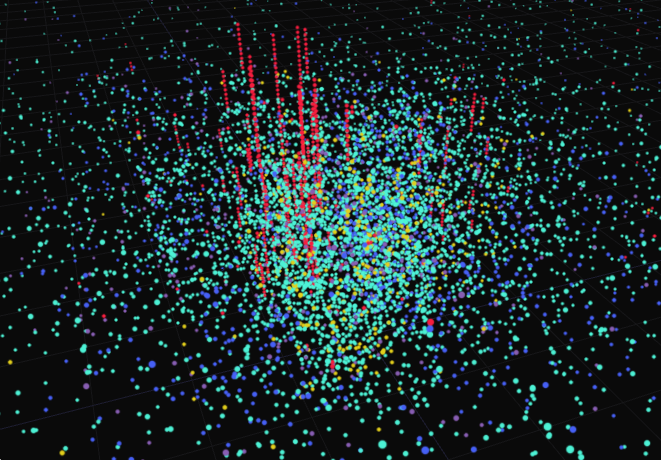
\includegraphics[width=0.8\textwidth]{images/bitnodes.png}
    \caption{Visualizzazione di una porzione di nodi attivi elaborati e classificati da \textit{Bitnodes} in base all'ultimo rilevamento online (i colori rappresentano il grado di sincronizzazione).}
    \source{Bitnodes}
\end{figure}
L'implementazione permette anche di definire sia la percentuale di nodi \textit{miner} presenti nella rete da simulare che gli hashrate associati ai peer.

\section{Mining}
La simulazione del processo di \textit{mining} dei nodi è modellata in modo tale che rispetti difficoltà ed andamento paragonabili a quelli reali ma senza l'esigenza computazionale e temporale richiesta dal protocollo Bitcoin. Nel protocollo Bitcoin i blocchi sono pubblicati e creati in un intervallo di tempo di circa $10$ minuti mentre all'interno della simulazione ogni step è considerato $1$ minuto. Dopo circa $10$ step un blocco è calcolato e propagato all'interno della rete. Per ovviare al problema dell'aumento dell'\textit{hashrate} dell'intera rete, Bitcoin implementa un meccanismo di \textit{difficoltà} secondo il quale ogni $2016$ blocchi la probabilità di trovare il \textit{nonce} corretto varia proporzionalmente alla potenza di calcolo dell'intera rete. Un maggior \textit{hashrate} comporta una frequenza nei blocchi minore di $10$ minuti e quindi, al successivo ricalcolo, la difficoltà risulterà proporzionalmente maggiore.\newline
Il valore della difficoltà \texttt{D} varia in base all'equazione \ref{eq:difficulty}; di conseguenza la probabilità di calcolo del \textit{nonce} corretto per un tempo \texttt{T} (minuti) è esponenziale:
\begin{equation}
    P = \exp^{-T/10}
\end{equation}
Ai fini della simulazione è interessante calcolare la probabilità di calcolo di un blocco data una percentuale di hashrate in un dato tempo $T$. Ogni \textit{miner} \texttt{m} possiede una frazione \texttt{h} della potenza di calcolo totale \texttt{H}; tramite la distribuzione di Poisson è possibile sapere quale è la probabilità che un nodo risolva il blocco in un dato tempo \texttt{T}:
\begin{equation}\label{eq:mining}
    P_m = \frac{(h * H / 100) * T}{(2^{32} * D)}
\end{equation}
Dove \texttt{D} è il valore della \textit{difficoltà} allo stato attuale della rete con un \textit{hashrate} totale \texttt{H} espresso in $G/s$ o $G/min$ (di conseguenza \texttt{T} è espresso in secondi o minuti). $2^{32}$ è il numero di possibili combinazioni utilizzate da \textit{Hashcash}.\newline
Utilizzando un \textit{ASIC} con potenza di calcolo di $13~TH/s$ (potenza di uno degli \textit{ASIC} più utilizzati: \textit{Antiminer S9}) la probabilità di calcolare un blocco in $10$ minuti è del $0.00000027295900726337\%$ (dati gli attuali valori di \texttt{H} e \texttt{D}, Novembre 2018).\newline
Conoscendo la distribuzione della probabilità nel tempo per ogni nodo è possibile evitare ogni tipo di attività di calcolo del \textit{nonce} tramite \textit{Hashcash} e facilitarne la simulazione: ad ogni step i \textit{miner} hanno una possibilità di calcolare e pubblicare un blocco data dall'equazione \ref{eq:mining}.
In quanto la rete Bitcoin risulta essere molto variabile spesso i valori \texttt{D} ed \texttt{H} non sono sempre bilanciati; in questo caso si dice che la rete non è in uno stato \textit{steady}. Con i precedenti valori di \texttt{D} e \texttt{H} infatti la probabilità $P_m$ è inferiore al $100\%$.
\begin{equation}
    P = H * 600 / (2^{32} * D) = 0.90972%
\end{equation}
Questo significa che il tempo medio per ogni blocco è superiore ai $10$ minuti e che la difficoltà va decrementata al successivo checkpoint.
Nel caso in cui la rete fosse bilanciata la probabilità di trovare un blocco utilizzando tutta la potenza di calcolo possibile dopo $10$ minuti è del $100\%$.
\begin{code}
    \captionof{listing}{Funzione di calcolo della probabilità \texttt{P} dato un tempo \texttt{T} e una percentuale di \textttt{H}.}
\begin{minted}{c}
double mining_probability(double hashrate, double time_min) {
    int t = (int)time_min % 10;
    t = t == 0 ? 10 : t;

    return(((hashrate * env_global_hashrate / 100.0) * t)
            / (HASHPOW * env_difficulty));
}
\end{minted}
Durante una simulazione è possibile quindi che il numero di blocchi generati in totale differisca dal numero previsto dalla divisione:
\begin{equation}
    numbero\_blocchi = tempo\_esecuzione/10
\end{equation}
\end{code}
\begin{figure}[H]
    \centering
    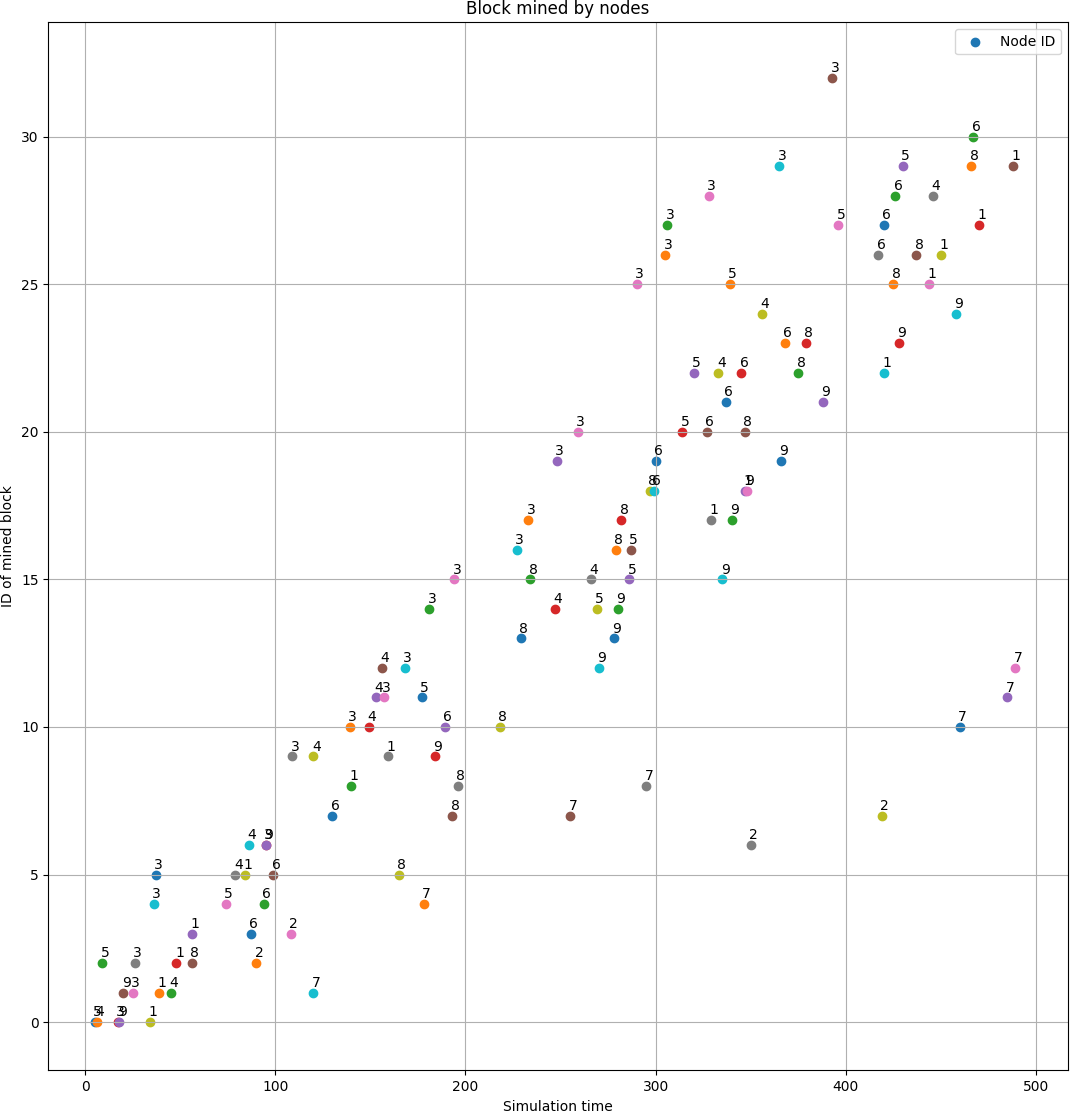
\includegraphics[width=0.8\textwidth]{images/blockmined.png}
    \caption{Visualizzazione dei blocchi creati da ogni nodo nel corso di una simulazione di test.}
\end{figure}

\section{Messaggi}
Ogni nodo della rete può inviare o ricevere messaggi in accordo con il proprio stato di ricezione o produzione. Non tutti i nodi producono delle transazioni o dei blocchi ad ogni istante di tempo e per questo è necessario che tutta le rete sia costantemente informata in caso di nuove informazioni pubblicate. Non appena un blocco è stato pubblicato, ad esempio, gli altri nodi devono poterlo ricevere per aggiungerlo alla blockchain e lavorare sul blocco successivo per poter ricevere il compenso. Al fine di rispondere a queste esigenze sono stati implementate alcune tipologie di messaggio che i nodi possono inviare o ricevere tramite \texttt{union}. Ogni messaggio ricevuto dai nodi è poi interpretato e gestito a seconda della tipologia.
\begin{code}
    \captionof{listing}{\texttt{union} dei tipi di messaggi scambiati tra i peer della rete.}
\begin{minted}{c}
union msg {
    char     type;
    LinkMsg  link;
    MigrMsg  migr;
    TransMsg trans;
    BlockMsg block;
    AskMsg   askblock;
};
\end{minted}
\end{code}
\begin{figure}[H]
    \centering
    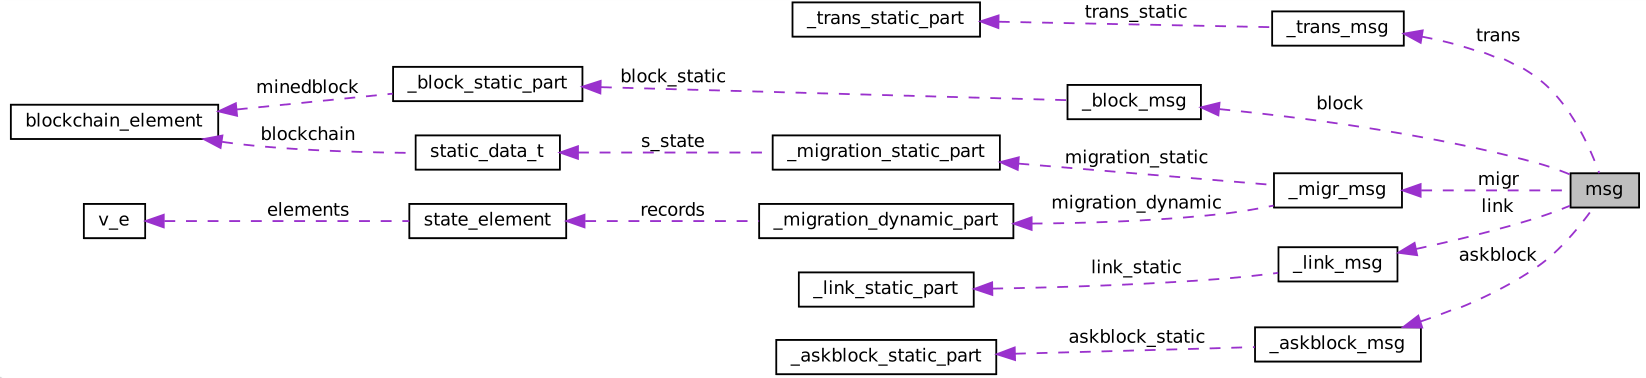
\includegraphics[width=\textwidth]{images/collaboration_union_msg.png}
    \caption{\textit{Collaboration diagram} per la struttura utilizzata per i messaggi.}
\end{figure}
Un messaggio può essere composto di una parte statica ed una dinamica. La parte statica è utilizzata per definire le caratteristiche del messaggio mentre la parte dinamica è utilizza per inserire informazioni aggiuntive che non sono state previste al momento della progettazione o che non sono classificabili in un singolo campo.\newline
I tipi di messaggi scambiati nel protocollo utilizzato nella blockchain simulata sono:
\begin{itemize}
    \item \texttt{TransMsg}: messaggio generato ed utilizzato per pubblicare una transazione nella rete;
    \item \texttt{BlockMsg}: messaggio creato ed utilizzato per pubblicare un blocco nella rete;
    \item \texttt{AskMsg}: messaggio di richiesta di determinato blocco.
\end{itemize}
Queste tipologie di messaggio non presentano una parte dinamica in quanto non è necessario utilizzare una struttura dati complessa: il protocollo simulato non necessita di tutte le caratteristiche presenti nel protocollo reale di Bitcoin. Durante l'utilizzo di un normale client Bitcoin, infatti, non sarà possibile vedere questi tipi di messaggi.\newline
I singoli campi del messaggio possono essere visti come elementi di un pacchetto IP. Il pacchetto contiene sia i dati che i dettagli utili per il routing.
\begin{code}
    \captionof{listing}{Struttura di un messaggio \texttt{TransMsg}.}
\begin{minted}{c}
struct _trans_static_part {
    char           type;          // Message type
    float          timestamp;     // Timestep of creation
    unsigned short ttl;           // Time-To-Live
    int            transid;       // Message Identifier
    int            from;          // ID of payer
    int            to;            // ID of payee
    unsigned int   creator;       // ID creator of the message
    unsigned int   num_neighbors; // Number of neighbors of forwarder
};

struct _trans_msg {
    struct  _trans_static_part trans_static;
} TransMsg;
\end{minted}
\end{code}
I campi comuni a tutti i messaggi sono:
\begin{itemize}
    \item \texttt{type}: utilizzato per definire il tipo del messaggio;
    \item \texttt{timestamp}: tempo di creazione del messaggio;
    \item \texttt{ttl}: \textit{Time-To-Live} utilizzato per evitare overhead nella rete;
    \item \texttt{num\_neighbors}: utilizzato dall'algoritmo di broadcast dipendente dal grado [\ref{app:sec:ddf}].
\end{itemize}
I campi specifici dei messaggi del protocollo invece riguardano:
\begin{itemize}
    \item \texttt{TransMsg}
    \begin{itemize}
        \item \texttt{transid}: identificativo della transazione;
        \item \texttt{from}: identificativo dell'utente che sta inviando denaro;
        \item \texttt{to}: identificativo dell'utente che sta ricevendo denaro;
    \end{itemize}
    \item \texttt{BlockMsg}
        \begin{itemize}
            \item \textit{minedblock}: informazioni sul blocco appena calcolato e le relative transazioni che contiene;
        \end{itemize}
    \item \texttt{AskMsg}
        \begin{itemize}
            \item \texttt{blockid}: indice del blocco (nella blockchain) che il nodo richiede.
        \end{itemize}
\end{itemize}
\begin{figure}[H]
    \centering
    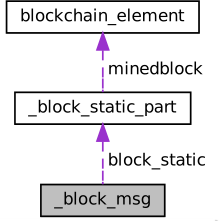
\includegraphics[width=0.3\textwidth]{images/collaboration_block.png}
    \caption{\textit{Collaboration diagram} per i messaggi \texttt{BlockMsg}}
\end{figure}

\section{Inizializzazione}
Il simulatore può astrarre da un grafo i nodi ed i collegamenti necessari a creare la rete dell'intera simulazione. Tramite \texttt{igraph} è possibile generare un file con la struttura della rete, ovvero, i link tra i vari nodi.
\begin{lstlisting}[frame=none,caption=Esempio di un file generato da \texttt{igraph} con $6$ nodi.]
graph {
  0;
  1;
  2;
  3;
  4;
  5;

0 -- 1;
0 -- 2;
1 -- 3;
1 -- 2;
3 -- 4;
3 -- 5;
}
\end{lstlisting}
I nodi della rete devono essere creati ed inizializzati secondo la struttura topologica definita dal file di configurazione.
Il simulatore deve essere istruito, quindi, a creare le \textit{hashtable} in cui inserire sia le entità gestite localmente all'interno del \textit{LP} che globali. L'inizializzazione infatti deve avvenire per tutti i nodi ed il \textit{SIMA} deve aver accesso a tutti i dati. Queste strutture dati sono di tipo \texttt{hash\_t} e contengono tutte le informazioni riguardanti i nodi.\newline
Prima di assegnare i nodi ai singoli \textit{LP} è fondamentale inizializzare \textit{GAIA} definendo il numero di \textit{LP}, il numero dei nodi e l'indirizzo utilizzato per la comunicazione (\texttt{GAIA\_Initialize}).
\begin{code}
    \captionof{listing}{Strutture dati utilizzate per rappresentare un nodo.}
\begin{minted}{c}
typedef struct hash_data_t {
    int           key;            // SE identifier
    int           lp;             // Logical Process ID
    double        hashrate;       // Hashrate of the node (if miner)
    int           attackerid;     // ID of the attacker
    int           miner;          // Boolean: is the node a miner?
    int           internal_timer; // Used to track mining activity
    int           latestblock;    // ID of the latest block
    static_data_t s_state;        // Static part of the SE local state
    GHashTable *  state;          // Local state as an hash table
                                  // (glib) (dynamic part)
    unsigned int  num_neighbors;  // Number of SE's neighbors
                                  // (dynamically updated)
} hash_data_t;

typedef struct hash_node_t {
    struct hash_data_t *data;
    struct hash_node_t *next;
} hash_node_t;

typedef struct hash_t {
    struct hash_node_t **bucket;
    int                  count;
    int                  size;
} hash_t;
\end{minted}
\end{code}
\begin{figure}[H]
    \centering
    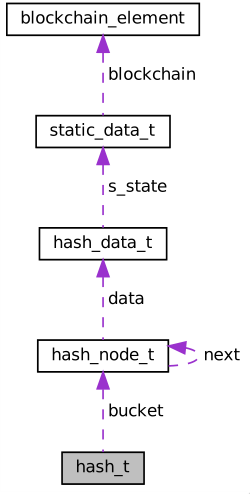
\includegraphics[width=0.3\textwidth]{images/collaboration_hasht.png}
    \caption{\textit{Collaboration diagram} per la struttura dati \texttt{hash\_t}}
\end{figure}
Una volta creati i vari nodi questi devono essere registrati tramite l'API \texttt{GAIA\_Register} così che possano essere gestiti dal middleware ed il \texttt{SIMA}. Una volta che i nodi sono stati assegnati agli \textit{LP} questi devono essere inizializzati e il grafo delle connessioni deve essere costruito.\newline
La funzione \texttt{lunes\_load\_graph\_topology} permette di leggere il file ed inizializzare una \textit{hashtable} per ogni \textit{SE}. Anche in questo caso ogni nodo è informato dai propri \textit{neighbor} tramite un messaggio di \texttt{link} (\texttt{L}). Ogni nodo ricevente aggiorna la propria lista di peer a cui è connesso e che dovrà utilizzare per scambiare informazioni con il resto della rete. L'evento generato dal messaggio \texttt{LinkMsg} è catturato dal nodo e gestito tramite la funzione \texttt{user\_link\_event\_handler}. Ad ogni nodo viene, quindi, assegnato un identificativo numerico ed una percentuale di hashrate (se si tratta di un nodo miner) in base alle condizioni previste dalla configurazione. L'assegnamento dell'hashrate per ogni nodo avviene tramite una funzione randomica \texttt{RND\_Interval} ed al fine di raggiungere una soglia pari al $100\%$ questi valori vengono normalizzati.
\begin{code}
    \captionof{listing}{Funzione di suddivisione in \texttt{n} nodi dell'hashrate in percentuale. Nel caso ci sia un attaccante la suddivisione dell'hashrate non considera quella prodotta dell'attaccante.}
\begin{minted}{c}
static void generate_hashrates(int n) {
    rates = (double *)malloc(n * sizeof(double));
    double sum          = 0;
    int    miners_count = MINERS_COUNT * n;
    for (int i = 0; i < miners_count; ++i) {
        double val = RND_Interval(S, 0.0, 100.0);
        sum     += val;
        rates[i] = val;
    }
    for (int i = 0; i < miners_count; i++) {
        rates[i] = rates[i] / sum * (100.0 - atk_hashrate);
    }
}
\end{minted}
\end{code}
Ogni nodo deve anche replicare la struttura dati di una blockchain per mantenere aggiornata la propria lista di blocchi e transazioni. La struttura dati della blockchain è inizialmente vuota e non sono stati previsti meccanismi di validazione tramite \textit{hashing} in quanto risulterebbe troppo dispendioso in termini di potenza computazionale e non necessario ai fini della simulazione. La blockchain è implementata come una lista contenuta nella parte statica del nodo: \texttt{s\_state}. Un blocco (un elemento della lista) contiene tutte le transazioni ricevute in una lista. I limiti della dimensione delle liste sono stati definiti prendendo il numero medio di transazioni per blocco nella reale rete dei Bitcoin ed un limite massimo di blocchi adatto ad eseguire la simulazione senza perdita di dati o eccessiva occupazione di memoria.
\begin{code}
    \captionof{listing}{}
\begin{minted}{c}
typedef struct blockchain_element {
    int         id;          // ID of the block
    int         latesttrans; // ID of the lastest transacation
    Transaction trans[1500]; // Mean # of transactions per block
} Block;

/* Static part of the SE state */
typedef struct static_data_t {
    char  changed;            // ON if there has been a state
                              // change in the last timestep
    char  freerider;          // 1 if free-rider, 0 not free-rider
    float time_of_next_trans; // Timestep in which the next new
                              // transaction will be created and sent
    float time_of_next_check; // Timestep in which the next check
                              // for new block will be created and sent
    Block blockchain[1500];   // Array of blocks
} static_data_t;
\end{minted}

\section{Interazione}
Una volta completata la fase di inizializzazione il simulatore può ricevere gli eventi inoltrati dal \texttt{SIMA} tramite \texttt{GAIA\_Receive}. Gli eventi gestiti sono di diverse tipologie:
\begin{itemize}
    \item \texttt{NOTIF\_MIGR}: una migrazione di un'entità locale deve essere gestita;
    \item \texttt{NOTIF\_MIGR\_EXT}: una migrazione deve essere eseguita ma non all'interno dell'attuale processo logico;
    \item \texttt{REGISTER}: una nuova \textit{simulated entity} deve essere registrata ma è ancora gestita da un altro processo logico;
    \item \texttt{EXEC\_MIGR}: una migrazione di una \textit{SE} in questo processo logico deve essere gestita, i dati sono copiati all'interno di strutture dati allocate per l'entità che deve essere migrata;
    \item \texttt{EOS} (\textit{End Of Step}): il corrente step della simulazione è terminato (è passata una unità di tempo);
    \item \texttt{UNSET}: è stato ricevuto un evento gestito all'interno delle singole entità (eventi creati all'interno della simulazione: \texttt{BlockMsg}, \texttt{TransMSg}, etc.).
\end{itemize}
I messaggi \texttt{EOS} ricevuti dal manager sono utilizzati per tener traccia del tempo, raccogliere statistiche da \textit{GAIA} e avviare un nuovo ciclo di esecuzione tramite la funzione \texttt{Generate\_Computation\_and\_Interactions}. Ad ogni nuovo ciclo vengono eseguite le routine di creazione di eventuale creazione dei messaggi che sono inviati e ricevuti a partire dal successivo step.\newline
I messaggi che compongono l'interazione tra i nodi sono gestiti nella funzione \texttt{user\_model\_events\_handler}. I messaggi di tipo \texttt{UNSET} costituiscono un wrapper dei messaggi scambiati tra i nodi. I simulatore si occupa di gestire i messaggi di tipo \texttt{UNSET} senza conoscerne il contenuto mentre ogni nodo è capace di elaborare solo i messaggi definiti dal programmatore in base al tipo definito all'interno del campo \texttt{type}.\newline
Poiché i nodi sono modellati tramite agenti, è necessario definirne il comportamento pro-attivo.\newline
I nodi abilitati al \textit{mining} devono ad ogni step tentare si calcolare un blocco. Se, tramite il calcolo della probabilità, il blocco è stato validato allora il nodo può inviarlo all'intera rete utilizzando un protocollo di \textit{broadcast}. Questo algoritmo genera un maggior overhead nella rete (messaggi ridondanti) ma garantisce una copertura più rapida. Questo comportamento è desiderabile in quanto:
\begin{enumerate}
    \item il nodo \textit{miner} che ha inviato il messaggio ha più possibilità che il blocco venga inserito nella blockchain più lunga per reclamare il reward;
    \item i nodi vicini possono aggiungere il blocco alla proprio blockchain ed iniziare senza attesa a calcolare il nuovo blocco;
    \item la ridondanza è azzerata poiché i nodi che non sono interessati lo scarteranno in quanto il blocco è identificato obsoleto; in questo caso il blocco si dice \textit{stale}.
\end{enumerate}
\begin{figure}[H]
    \centering
    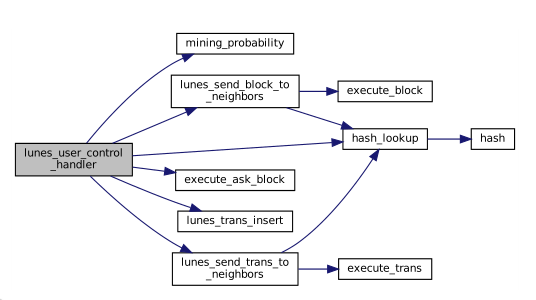
\includegraphics[width=\textwidth]{./images/graphcall_node_routine.png}
    \caption{Diagramma delle chiamate a funzione eseguite durante un ciclo di esecuzione di un nodo.}
\end{figure}
Nel caso in cui invece il nodo \textit{miner} non riesca a validare il blocco in questo step allora verrà inviata una richiesta ai proprio \textit{neighbors} di eventuali aggiornamenti sulla blockchain tramite il messaggio \texttt{AskMsg}. Questo messaggio non è inoltrato dagli altri nodi e può non ricevere una risposta. La semantica della richiesta è: 
\begin{itemize}
    \item il nodo $a$, \textit{miner}, sta lavorando sul blocco di indice $x$ e tramite un messaggio \texttt{AskMsg} chiede ai nodi vicini se quel nodo è già stato validato e distribuito nella rete;
    \item se la blockchain in possesso dai vicini ha lunghezza almeno $x+1$ allora il nodo $a$ è aggiornato tramite un messaggio \texttt{BlockMsg}.
\end{itemize}
Questo comportamento potrebbe causare un notevole overhead nella rete, infatti è limitato secondo una funzione di probabilità esponenziale, ma simula un normale decorso di un nodo che si connette alla rete. Ogni \textit{full node} che vuole far parte della rete Bitcoin attuale deve chiedere ai propri \textit{peer} tutti i blocchi della blockchain per poter iniziare a validare transazione e blocchi.\newline
Tutti i nodi, invece, possono creare e pubblicare delle transazioni tramite \texttt{TransMsg}. Il nodo che ha creato una transazione inserisce la stessa all'interno dell'attuale blocco e la propaga, tramite l'algoritmo di broadcast dipendente dal grado, ai nodi vicini. I nodi che ricevono il messaggio \texttt{TransMsg} devono validare la transazione: se la transazione fa già parte della blockchain allora viene rifiutata ed il messaggio non è inoltrato. Una volta che una transazione è inserita nella blockchain di un blocco il messaggio \texttt{TransMsg} viene inoltrato ai vicini.
\begin{figure}[H]
    \centering
    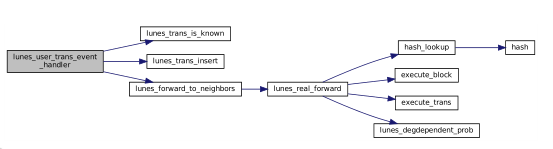
\includegraphics[width=\textwidth]{./images/graphcall_trans.png}
    \caption{Diagramma delle chiamate a funzione eseguite durante la ricezione di un messaggio \texttt{TransMsg}.}
\end{figure}

\section{Realizzazione}
L'implementazione dei test con i vari scenari di attacco è stata effettuata in \textit{C} utilizzando le API messe a disposizione da \textit{GAIA} tramite \textit{LUNES}.\newline
L'utilizzo di molteplici \texttt{struct} annidate permette di avere una alta configurabilità delle entità del sistema e modularità, a discapito però della leggibilità. L'intera progettazione è avvenuta per fasi: la prima fase ha avuto come obiettivo la creazione di un sistema che simulasse una blockchain; la seconda fase ha imposto alcuni vincoli al sistema per modellarlo come la blockchain Bitcoin; l'ultima fase ha raccolto l'Implementazione dei vari test di attacco.\newline
La divisione in fasi distinte ha permesso al sistema di crescere senza l'ausilio sovrastrutture garantendo una alta modularità.\newline
I parametri di configurazione della rete, dei nodi, dei test e degli algoritmi di propagazione sono gestiti esternamente tramite variabili d'ambiente del sistema. Questo permette di evitare modifiche al codice e compilazione durante molteplici esecuzioni.\newline

% NeoTex: mainfile=main.tex:
